\section{Spatial Econometrics} 

\subsection{Background} 

\begin{frame}
	\frametitle{Spatial Econometric Tools}
 \begin{itemize}
 \item Not much commercially available
 \item Many specialized scripts
 \begin{itemize}
 \item Stata, SAS, SPSS, etc.
 \end{itemize}
 \item Toolboxs and libraries
 \begin{itemize}
 \item R: spdep, sphet
 \item MatLab: Econometrics Toolbox
 \end{itemize}
 \end{itemize}
 \end{frame} 

\begin{frame}
	\frametitle{Econometrics in Python -- Currently}
  \begin{quote}
  ``Since there is no free programming language that can be
  considered a \emph{lingua franca} of applied econometrics, choosing
  Python and writing or translating econometric routines may be
  worth the effort.''
  \end{quote}
  \qquad\qquad\qquad\qquad -- C. Choirat and R. Seri (2009), J. Appl. Econ.
 \end{frame} 

\begin{frame}
	\frametitle{Econometrics in Python -- Options}
 \begin{itemize}
 \item pyGauss
 \item pyTrix
 \item EconPy
 \item statsmodels / pandas
 \end{itemize}
 \end{frame} 

\begin{frame}
	\frametitle{Immediate Plan}
 \begin{itemize}
 \item OLS estimation with diagnostics for spatial effects
 \item 2SLS estimation with diagnostics for spatial effects
 \item Spatial 2SLS for spatial lag model (with endogeneity)
 \item GM and GMM estimation for spatial error model
 \item GMM spatial error with heteroskedasticity
 \item Spatial HAC estimation
 \end{itemize}
 \end{frame} 

\begin{frame}
	\frametitle{Challenges}
 \begin{itemize}
 \item Handle large problems
 \item Efficient spatial weights
 \item Modularity and reusability
 \end{itemize}
 \end{frame} 

\begin{frame}
	\frametitle{Functionality}
 \begin{itemize}
 \item Spatial weights creation
 \item Spatially lagged variable computation
 \item GMM estimation methods
 \item Diagnostics
 \item Allow endogeneity
 \end{itemize}
 \end{frame} 

\begin{frame}
	\frametitle{Delivery}
 \begin{itemize}
 \item Freestanding $\rightarrow$ GeoDaSpace
 \item Command line $\rightarrow$ PySAL
 \item ArcGIS toolbox
 \end{itemize}
 \end{frame} 

\subsection{PySAL} 

\begin{frame}
	\frametitle{PySAL Econometrics -- Setup OLS}
 \VerbatimInput[frame=single,numbers=left,numbersep=3pt,
 fontsize=\small]{figures/ols_commandLine.txt}
 \end{frame} 

\begin{frame}
	\frametitle{PySAL Econometrics -- Diagnostics Summary}
  \begin{center}
  \includegraphics<1->[width=0.53\linewidth]{ols_summary.png}%
  \end{center}
 \end{frame} 

\begin{frame}
	\frametitle{PySAL Econometrics -- Individual Diagnostics}
 \VerbatimInput[frame=single,numbers=left,numbersep=3pt,
 fontsize=\small]{figures/ols_diag.txt}
 \end{frame} 

\begin{frame}
	\frametitle{PySAL Econometrics -- Spatial Diagnostics}
 \VerbatimInput[frame=single,numbers=left,numbersep=3pt,
 fontsize=\small]{figures/spatial_diag.txt}
 \end{frame} 

\begin{frame}
	\frametitle{PySAL Econometrics -- Setup S2SLS}
 \VerbatimInput[frame=single,numbers=left,numbersep=3pt,
 fontsize=\small]{figures/s2sls_setup.txt}
 \end{frame} 

\begin{frame}
	\frametitle{PySAL Econometrics -- Setup GSLS (KP 1998, 1999)}
 \VerbatimInput[frame=single,numbers=left,numbersep=3pt,
 fontsize=\small]{figures/gsls_setup.txt}
 \end{frame} 

\subsection{GeoDaSpace} 

\begin{frame}
	\frametitle{Loosely Coupled Framework}
  \begin{center}
  \includegraphics<1->[width=0.70\linewidth]{software_links.png}%
  \end{center}
 \end{frame} 

\begin{frame}
	\frametitle{User Interface}
  \begin{center}
  \includegraphics<1->[width=0.60\linewidth]{space1.png}%
  \llap{\includegraphics<2->[width=0.60\linewidth]{space2.png}}%
  \llap{\includegraphics<3->[width=0.50\linewidth]{spaceW.png}}%
  \llap{\includegraphics<4->[width=0.60\linewidth]{space3.png}}%
  \llap{\includegraphics<5->[width=0.20\linewidth]{spaceL.png}}%
  \llap{\includegraphics<6->[width=0.60\linewidth]{space4.png}}%
  \llap{\includegraphics<6->[width=0.20\linewidth]{spaceL.png}}%
  \llap{\includegraphics<7->[width=0.60\linewidth]{space5.png}}%
  \llap{\includegraphics<8->[width=0.80\linewidth]{spaceR.png}}%
  \llap{\includegraphics<9->[width=0.60\linewidth]{space4.png}}%
  \end{center}
 \end{frame} 

\begin{frame}
	\frametitle{(Near) Future}
 \begin{itemize}
 \item Spatial regimes
 \item Probit (classic and spatial)
 \item Maximum Likelihood
 \item Panel data
 \end{itemize}
 \end{frame} 



\section{Conclusion} 

\subsection{Next Steps} 

\begin{frame}
	\frametitle{PySAL Release Schedule}
	\begin{block}{6 month release cycle}
 \begin{itemize}
 \item 1.0 - August 1, 2010
        \begin{itemize}
	  \item (700+ downloads since)
	\end{itemize}
 \item 1.1 - January 31, 2011
        \begin{itemize}
	  \item Spatial Dynamics
	  \item Space-Time Event Clustering
	  \item \alert{Spatial Econometrics}
	\end{itemize}
\item 2.0 - August 1, 2011
 \end{itemize}
 \end{block}
 \end{frame} 

\begin{frame}
	\frametitle{Other GeoDa Center Software}
 
\begin{block}{Currently Available}
 \begin{itemize}
 \item PySAL
 \item GeoDa (legacy)
 \item OpenGeoDa
 \item STARS
 \end{itemize}
 \end{block} 
\begin{block}{Coming Soon}
 \begin{itemize}
 \item GeoDaSpace
 \item GeoDaNet
 \item GeoDaWeight
 \item dynTM
 \end{itemize}
 \end{block} \end{frame} 

\begin{frame}
	\frametitle{Questions}
  \begin{center}
 \begin{figure}[htbp]
 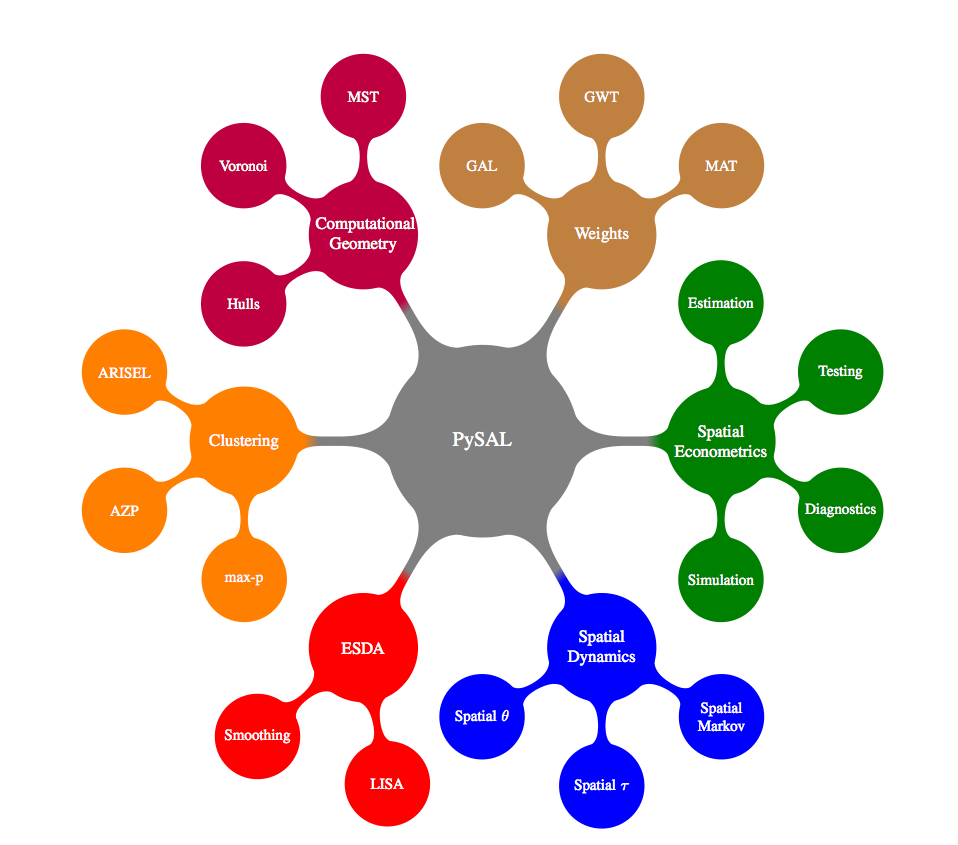
\includegraphics[width=0.60\linewidth]{pysalGraphic.png}
 \end{figure}
  {\color{blue}{\Large{geodacenter.asu.edu}}}\\
  {\color{blue}{\Large{www.pysal.org}}}
 \end{center}
 \end{frame} 



